\documentclass[class=report, crop=false, 12pt,a4paper]{standalone}
\usepackage{enumitem}
\usepackage{multicol}
\usepackage{graphicx}
\usepackage{float}
\usepackage{amsmath}
\usepackage{amssymb}
\usepackage{mathtools}
\usepackage{siunitx}
\usepackage{commath}
\usepackage{array}
\usepackage{natbib}
\usepackage{cancel}
\usepackage[a4paper,width=150mm,top=25mm,bottom=25mm]{geometry}
\setlength{\parindent}{0pt}
\begin{document}
\section{Thin-walled cylinders}
\textbf{Thin walled cylinders} have a wall thickness $t$ much smaller than the cylinder radius $R$ (at least one twentieth).
\begin{figure}[H]
    \centering
    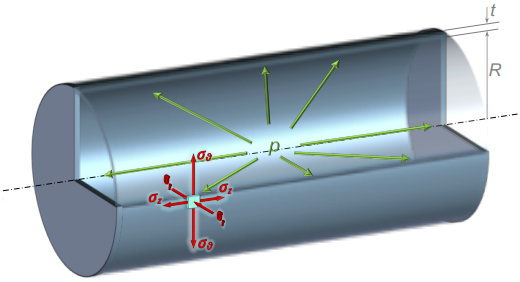
\includegraphics[height = 5cm]{../img/diagram102.png}
    \caption{}
\end{figure}
The \textbf{hoop stresses} $\sigma_{\theta}$ can be considered \textbf{constant} across the wall thickness $t$. The \textbf{radial stresses} $\sigma_t$ is \textbf{negligible} in comparison to the hoop stresses $\sigma_{\theta}$. Under these conditions, the state of stress at each point of the cylinder can be estimated to good accuracy by simple equilibrium considerations. 
\begin{figure}[H]
    \centering
    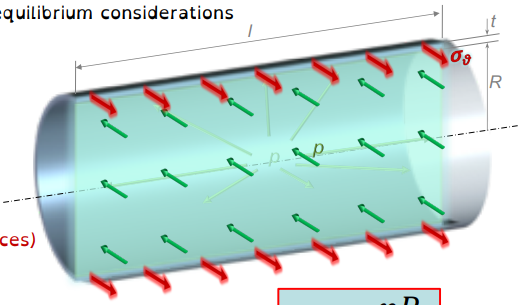
\includegraphics[height = 5cm]{../img/diagram103.png}
    \caption{Hoop stress - equilibrium of transversal forces.}
\end{figure}
\begin{gather}
    p\cdot l \cdot 2R = 2 \left(\sigma_{\theta} t l\right)
    \sigma_{\theta} = \frac{p R}{t}
\end{gather}
Under these conditions, the state of stress at each point of the cylinder can be estimated to good accuracy by simple equilibrium considerations. 
\begin{figure}[H]
    \centering
    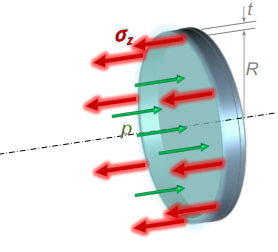
\includegraphics[height = 5cm]{../img/diagram104.png}
    \caption{Longitudinal stress - equilibrium of axial forces.}
\end{figure}
\begin{gather}
    p \cdot \pi R^2 = \sigma_z \cdot 2 \pi R \cdot t\\
    \sigma_z = \frac{pR}{2t}
\end{gather}
\begin{figure}[H]
    \centering
    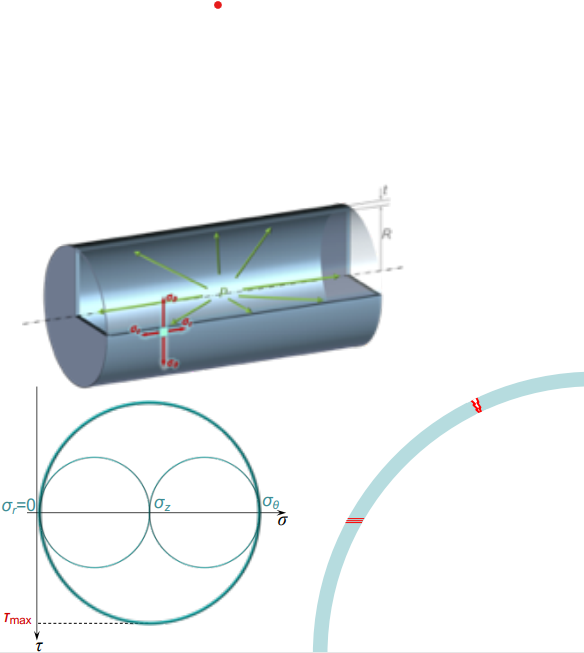
\includegraphics[height = 7cm]{../img/diagram105.png}
    \caption{}
\end{figure}
\begin{align}
    \sigma_{\theta} &= \frac{pR}{t}\\
    \sigma_z &= \frac{pR}{2t} = \frac{\sigma_{\theta}}{2}
\end{align}
\section{Thick-walled cylinders - radial and hoop\\ stresses}
\subsection{Failure of thick wall cylinders}
\begin{figure}[H]
    \centering
    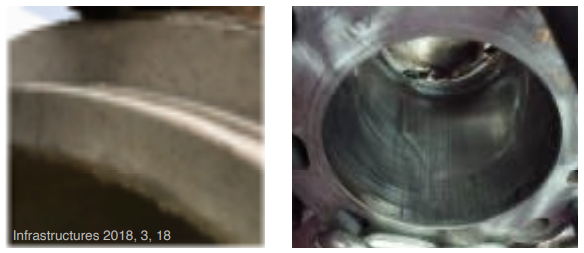
\includegraphics[height = 5cm]{../img/diagram106.png}
    \caption{}
\end{figure}
When thickness increases with respect to radius, the radial variation of hoop stress becomes considerable and the radial stress is no longer available.
\subsection{Radial and hoop stresses \& strains}
For the determination of radial and circumferential stresses and strains, equilibrium equations on their own are not sufficient.
\subsection{Solid mechanics equations}
\begin{figure}[H]
    \centering
    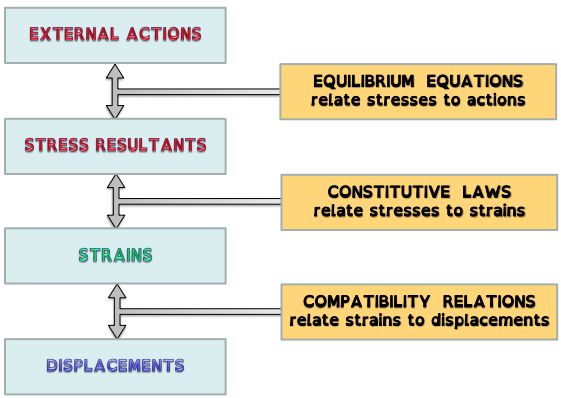
\includegraphics[height = 5cm]{../img/diagram107.png}
    \caption{}
\end{figure}
\subsection{Assumptions}
For long cylinder , far from the ends, we can assume that the deformation of the cylinder is symmetrical respect to the axis:
\begin{itemize}
    \item Cross-sections remain plane when subjected to pressure: longitudinal strain $\epsilon_z$ is independent of radius. i.e. $\epsilon_z =$ constant
    \item Displacements in each cross-section are purely radial
    \item Displacement is constant with circumferential co-ordinate and varies only with radial co-ordinate i.e. $u=f(r)$
    \item $\sigma_r$, $\sigma_{\theta}$ and $\sigma_z$ are principal stress
    \item Cross-sections remain plane when subjected to pressure: longitudinal strain $\epsilon_z$ is independent of radius. i.e. $\epsilon_z =$ constant
\end{itemize}
\begin{figure}[H]
    \centering
    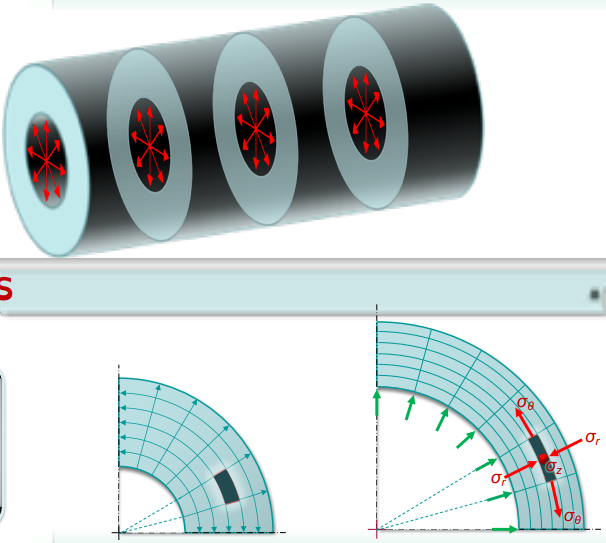
\includegraphics[height = 7cm]{../img/diagram108.png}
    \caption{}
\end{figure}
\subsection{Equilibrium equations}
\begin{figure}[H]
    \centering
    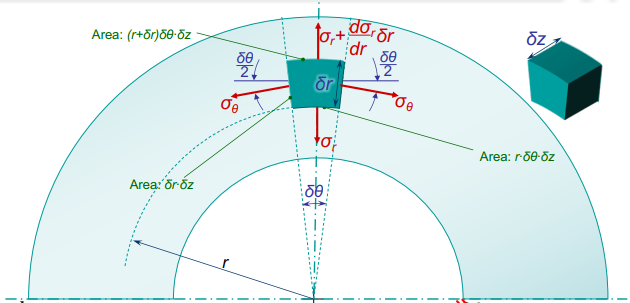
\includegraphics[height = 7cm]{../img/diagram109.png}
    \caption{}
\end{figure}
The equilibrium of radial forces is given by the following equation:
\begin{gather}
    -\sigma_r \left(r\cdot \cancel{\delta \theta} \cdot \cancel{\delta z}\right) + \left(\sigma_r + \frac{\dif \sigma_r}{\dif r}\delta r \right) \left[ \left(r + \delta r \right) \cdot \cancel{\delta \theta} \cdot \cancel{\delta z}\right] - \cancel{2} \sigma_{\theta} \left(\delta r \cdot \cancel{\delta z}\right) \cdot \cancel{\sin} \frac{\cancel{\delta \theta}}{\cancel{2}} = 0\\
    \rightarrow \cancel{-\sigma_r r} + \cancel{\sigma_r r} + \sigma_r \cancel{\delta r} + r \frac{\dif \sigma_r}{\dif r} \cancel{\delta r} + \cancel{\frac{\dif \sigma_r}{\dif r}\delta r^2} - \sigma_{\theta} \cancel{\delta r} = 0\\
    \rightarrow \sigma_r + r\frac{\dif \theta_r}{\dif r} - \sigma_{\theta} = 0
\end{gather}
\subsection{Compatibility relations}
\begin{figure}[H]
    \centering
    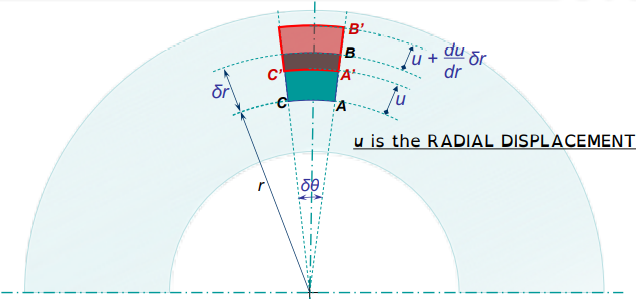
\includegraphics[height = 7cm]{../img/diagram110.png}
    \caption{}
\end{figure}
The radial strain is given by the following equation:
\begin{gather}
    \epsilon_r = \frac{\overline{A'B'} - \overline{AB}}{\overline{AB}}
\end{gather}
with: 
\begin{equation}
    \overline{AB} = \delta r
\end{equation}
and 
\begin{equation}
    \overline{A'B'} = \overline{AB} + \overline{BB'} - \overline{AA'} = \delta r + \left(\cancel{u} + \frac{\dif u}{\dif r} \delta r \right) - \cancel{u} = \delta r + \frac{\dif u}{\dif r} \delta r
\end{equation}
Leading to:
\begin{gather}
    \varepsilon_r = \frac{\left(\cancel{\delta r}+ \frac{\dif u }{\dif r} \cancel{\delta r}\right) - \cancel{\delta r}}{\cancel{\delta r}}\\
    \varepsilon_{\theta} = \frac{u}{r}
\end{gather}
\subsection{Constitutive laws}
Uniaxial:
\begin{equation}
    \begin{array}{l}
        \varepsilon_1 = \frac{\sigma_1}{E}\\
        \varepsilon_2 = -v\varepsilon_1\\
        \varepsilon_3 = -v\varepsilon_1
    \end{array} \hspace{1cm}
    \begin{array}{l}
        \sigma_1 = E\varepsilon_1\\
        \sigma_2 = 0\\
        \sigma_3 = 0
    \end{array}
\end{equation}
Biaxial:
\begin{equation}
    \begin{array}{l}
        \varepsilon_1 = \frac{1}{E} \left(\sigma_1 - v\sigma_2\right)\\
        \varepsilon_2 = \frac{1}{E} \left(\sigma_2 - v\sigma_1\right)\\
        \varepsilon_3 = -\frac{v}{E} \left(\sigma_1 + \sigma_2\right)        
    \end{array} \hspace{1cm}
    \begin{array}{l}
        \sigma_1 = \frac{E}{1-v^2} \left(\varepsilon_1 + v\varepsilon_2\right)\\
        \sigma_2 = \frac{E}{1-v^2} \left(\varepsilon_2 + v\varepsilon_1\right)\\
        \sigma_3 = 0        
    \end{array}
\end{equation}
Triaxial:
\begin{equation}
    \begin{array}{l}
        \varepsilon_1 = \frac{1}{E}\left[\sigma_1 - v\left(\sigma_2 + \sigma_3\right)\right]\\
        \varepsilon_2 = \frac{1}{E}\left[\sigma_2 - v\left(\sigma_3 + \sigma_1\right)\right]\\
        \varepsilon_3 = \frac{1}{E}\left[\sigma_3 - v\left(\sigma_1 + \sigma_2\right)\right]
    \end{array} \hspace{1cm} 
    \begin{array}{l}
        \sigma_1 = \frac{E}{\left(1+v\right)\left(1-2v\right)} \left[\left(1-v\right)\varepsilon_1 + v\left(\varepsilon_2 + \varepsilon_3\right)\right]\\
        \sigma_2 = \frac{E}{\left(1+v\right)\left(1-2v\right)} \left[\left(1-v\right)\varepsilon_2 + v\left(\varepsilon_1 + \varepsilon_3\right)\right]\\
        \sigma_3 = \frac{E}{\left(1+v\right)\left(1-2v\right)} \left[\left(1-v\right)\varepsilon_3 + v\left(\varepsilon_1 + \varepsilon_2\right)\right]
    \end{array}
\end{equation}
The analytical solution of the stress distribution is possible, in simple form, only in the \textit{case of biaxial state of stress}.
\subsubsection{Cylinders with internal pressure}
A pressure difference can be maintained inside the cylinder in one of the following methods:
\begin{figure}[H]
    \centering
    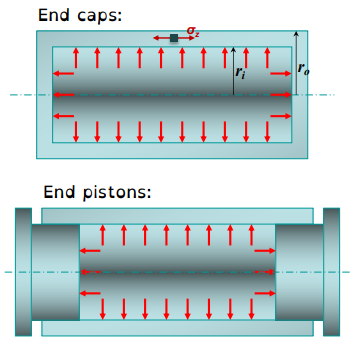
\includegraphics[height = 5cm]{../img/diagram111.png}
    \caption{}
\end{figure}
Only in the case of end pistons, can we find an analytical solution for the stress distributions in thick cylinders: no axial force acts on the cylinder and the state of stress is plane.
\begin{figure}[H]
    \centering
    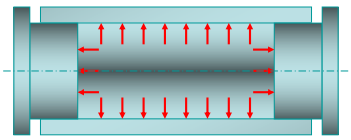
\includegraphics[height = 3cm]{../img/diagram112.png}
    \caption{}
\end{figure}
\subsubsection{Plane stress state}
Biaxial:
\begin{equation}
    \begin{array}{l}
        \varepsilon_1 = \frac{1}{E} \left(\sigma_1 - v\sigma_2\right)\\
        \varepsilon_2 = \frac{1}{E} \left(\sigma_2 - v\sigma_1\right)\\
        \varepsilon_3 = -\frac{v}{E} \left(\sigma_1 + \sigma_2\right)        
    \end{array} \hspace{1cm}
    \begin{array}{l}
        \sigma_1 = \frac{E}{1-v^2} \left(\varepsilon_1 + v\varepsilon_2\right)\\
        \sigma_2 = \frac{E}{1-v^2} \left(\varepsilon_2 + v\varepsilon_1\right)\\
        \sigma_3 = 0        
    \end{array}
\end{equation}
\subsubsection{Cylindrical}
In the biaxial case, in a cylindrical coordinate system $r, \, \theta, ,\ z$.
\begin{equation}
    \begin{array}{l}
        \varepsilon_r = \frac{1}{E} \left(\sigma_r - v\sigma_{\theta}\right)\\
        \varepsilon_{\theta} = \frac{1}{E} \left(\sigma_{\theta} - v\sigma_r\right)\\
        \varepsilon_z = -\frac{v}{E} \left(\sigma_r + \sigma_{\theta}\right)
    \end{array} \hspace{1cm} 
    \begin{array}{l}
        \sigma_r = \frac{E}{1-v^2}\left(\varepsilon_r + var\right)\\
        \sigma_{\theta} = \frac{E}{1-v^2} \left(\varepsilon_{\theta} + v \varepsilon_r\right)\\
        \sigma_z = 0
    \end{array}
\end{equation}
\subsection{Solid mechanics equations}
Equilibrium equations relate stresses to actions:
\begin{align}
    \frac{\dif \theta_r}{\dif r} + \frac{\sigma_r - \sigma_{\theta}}{r} = 0
\end{align}
Constitutive laws relate stresses to strains:
\begin{align}
    \sigma_r &= \frac{E}{1-v^2}\left(\varepsilon_r + v \varepsilon_{\theta}\right)\\
    \sigma_{\theta} &= \frac{E}{1-v^2}\left(\varepsilon_{\theta}+v\varepsilon_{r}\right)
\end{align}
Compatibility relations relate strains to displacements:
\begin{align}
    \varepsilon_r &= \frac{\dif u}{\dif r}\\
    \varepsilon_{\theta} &= \frac{u}{r}
\end{align}
Combining the equations together, we arrive at Euler's differential equation:
\begin{align}
    \frac{\dif^2 u}{\dif r^2} + \frac{1}{r}\cdot\frac{\dif u}{\dif r} - \frac{u}{r^2} &= 0\\
    r^2 u'' + r u' - u &= 0
\end{align}
Euler's differential equation is characterised by the fact that its coefficients depend on the variable $r$. The general solution to Euler's differential equation is:
\begin{align}
    u &= Ar + \frac{B}{r}
    u' &= A - \frac{B}{r^2} 
\end{align}
The constitutive laws hence become:
\begin{align}
    \sigma_r &= \frac{E}{1-v^2}\left(\frac{\dif u}{\dif r} + v \frac{u}{r}\right)\\
    \sigma_{\theta} &= \frac{E}{1-v^2}\left(\frac{u}{r}+v\frac{\dif u}{\dif r}\right)\\
    \sigma_r &= \frac{E}{1-v^2}\left[A - \frac{B}{r^2} + v\left(A + \frac{B}{r^2}\right)\right] = C - \frac{D}{r^2}\\
    \sigma_{\theta} &= \frac{E}{1-v^2} \left[A + \frac{B}{r^2} + v\left(A-\frac{B}{r^2}\right)\right] = C + \frac{D}{r^2}
\end{align}
Note that:
\begin{align}
    \sigma_r + \sigma_{\theta} = 2C = \textrm{const}
\end{align}
\subsubsection{Boundary conditions}
\begin{align}
    \sigma_r &= C - \frac{D}{r^2} = \frac{p_i r_i^2 - p_0r_0^2}{r_0^2 - r_i^2} - \frac{\left(p_i-p_0\right)r_i^2r_0^2}{\left(r_0^2-r_i^2\right)r^2}\\
    \sigma_{\theta} &= C + \frac{D}{r^2} = \frac{p_i r_i^2 - p_0r_0^2}{r_0^2 - r_i^2} + \frac{\left(p_i-p_0\right)r_i^2r_0^2}{\left(r_0^2-r_i^2\right)r^2}
\end{align}
If we have an internal pressure '$p_i$' and an external pressure is '$p_0$':
\begin{align}
    \sigma_r\left(r_i\right) &= -p_i = C - \frac{D}{r_i^2}\\
    C &= \frac{p_i r_i^2 - p_0r_0^2}{r_0^2 - r_i^2}\\
    \sigma_r\left(r_i\right) &= -p_0 = C - \frac{D}{r_0^2}\\
    D &= \frac{\left(p_i-p_0\right)r_i^2r_0^2}{\left(r_0^2-r_i^2\right)r^2}
\end{align}
\subsubsection{Radial and hoop stresses}
Lame's equations
\begin{align}
    \sigma_r &= \frac{p_i r_i^2 - p_0r_0^2}{r_0^2 - r_i^2} - \frac{\left(p_i-p_0\right)r_i^2r_0^2}{\left(r_0^2-r_i^2\right)r^2}\\
    \sigma_{\theta} &= \frac{p_i r_i^2 - p_0r_0^2}{r_0^2 - r_i^2} + \frac{\left(p_i-p_0\right)r_i^2r_0^2}{\left(r_0^2-r_i^2\right)r^2}
\end{align}
\subsection{Stress variation}
\subsubsection{General case}
\begin{figure}[H]
    \centering
    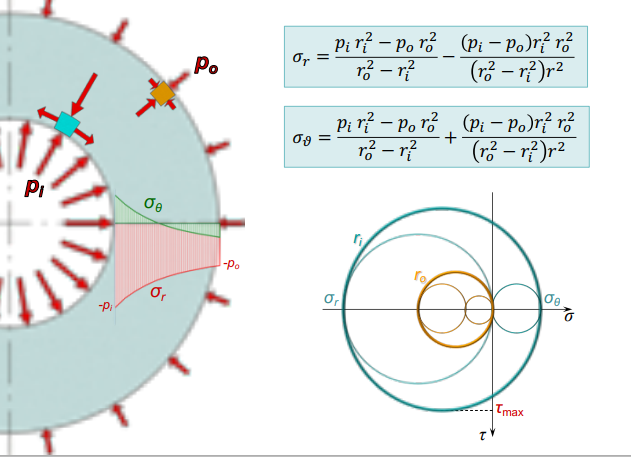
\includegraphics[height = 7cm]{../img/diagram113.png}
    \caption{}
\end{figure}
\subsubsection{$p_i$ only}
\begin{figure}[H]
    \centering
    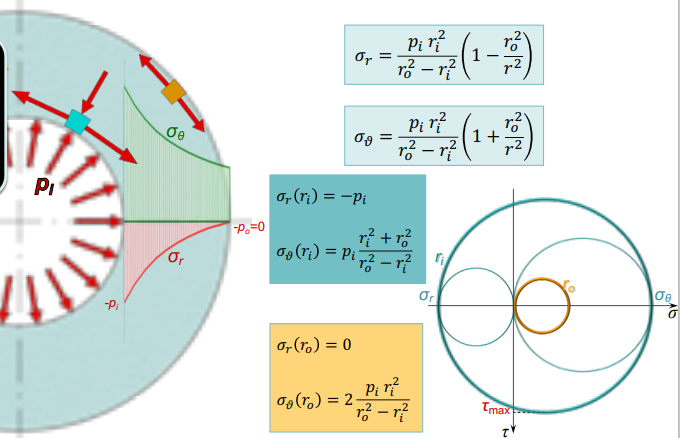
\includegraphics[height = 7cm]{../img/diagram114.png}
    \caption{}
\end{figure}
\subsubsection{$p_0$ only}
\begin{figure}[H]
    \centering
    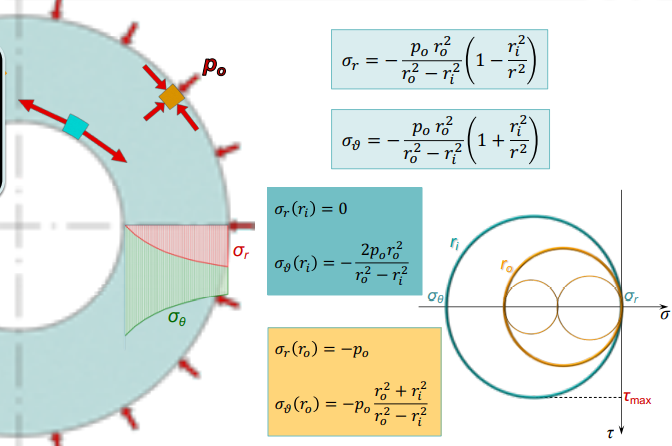
\includegraphics[height = 7cm]{../img/diagram115.png}
    \caption{}
\end{figure}
\section{Thick-walled cylinders - longitudinal stress}
\subsection{Cylinders with end-caps}
How do we deal with the case of end caps pistons? (Triaxial stress state)
\end{document}